% This file is part of Oaklisp.
%
% This program is free software; you can redistribute it and/or modify
% it under the terms of the GNU General Public License as published by
% the Free Software Foundation; either version 2 of the License, or
% (at your option) any later version.
%
% This program is distributed in the hope that it will be useful,
% but WITHOUT ANY WARRANTY; without even the implied warranty of
% MERCHANTABILITY or FITNESS FOR A PARTICULAR PURPOSE.  See the
% GNU General Public License for more details.
%
% The GNU GPL is available at http://www.gnu.org/licenses/gpl.html
% or from the Free Software Foundation, 59 Temple Place - Suite 330,
% Boston, MA 02111-1307, USA


\chapter{Sequences} \label{Sequences}

Sequences are manipulated using the \df{nth} operation, which is
settable (and locatable).  The sequence heirarchy is shown in
figure~\ref{fig:seqhier}.

\index{\texttt{sequence}}
\index{\texttt{vector-type}}
\index{\texttt{simple-vector}}
\index{\texttt{list-type}}
\index{\texttt{string}}
\index{\texttt{pair}}
\index{\texttt{null-type}}
\index{\texttt{cons-pair}}
\index{\texttt{lazy-cons-pair}}

\begin{figure}[h]
\centering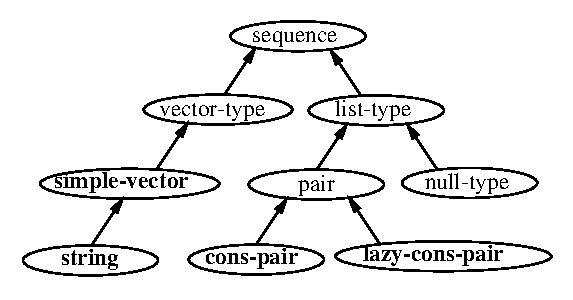
\includegraphics{seqhier}
\caption{The sequence type hierarchy.  Abstract types are in plain face
and instantiable ones in bold.} \label{fig:seqhier}
\end{figure}

\section{Type Predicates}

\pr{sequence?}{object}
\pr{vector?}{object}
\pr{string?}{object}
\pr{list?}{object}
\pr{pair?}{object}
\pr{null?}{object}
\pr{atom?}{object}


\section{Sequence Operations}

These operations work on all sequences.

\op{length}{list}
\lo{nth}{list n}
\lo{last}{list}
\lo{tail}{list n}
\op{copy}{sequence}

\op{append}{sequence1 sequence2}
\doc{Returns a sequence of the type of \emph{sequence1}.  One slight
bug is that one may not pass \df{append} a first argument that's a
list and a second that's not.  This may be fixed in the future.  All
other combinations should work correctly.}
\op{append\protect\bang}{sequence1 sequence2}
\doc{Most sequences have immutable lengths, and hence are not
appropriate arguments to \df{append\protect\bang}.  The major exception is lists.
The same bug is present here as in \df{append}.}

\op{reverse}{sequence}
\op{reverse\protect\bang}{sequence}

Some mapping operations are also applicable to sequences, and are
documented in Section~\ref{sec:controlmap}.

\section{Vector Constructors}

\op{vector}{\dt objects}
\doc{Returns a \df{simple-vector} containings \emph{objects}.}
\makin{simple-vector}{length}
\coercer{simple-vector}{sequence}


\section{List Constructors}

\op{list}{\dt objects}
\makin{list-type}{length fill-value}
\coercer{list-type}{sequence}
\op{cons}{object1 object2}
\makin{lazy-cons-pair}{car-thunk cdr-thunk}
\mc{lcons}{car-form cdr-form}
\doc{\macdef{}{(make lazy-cons-pair (lambda () \emph{car-form}) (lambda
() \emph{cdr-form}))}}


\section{List Accessors}

\lo{car}{pair}
\lo{cdr}{pair}
\lo{c$[$ad$]^{*}$r}{pair}
\doc{Actually these are only provided for up to four \texttt{a}'s and
\texttt{d}'s.  If you think you need more, you should probably be
defining accessor functions or using \df{nth} or perhaps
\df{destructure}.}
\lo{last-pair}{pair}
\doc{Takes successive \df{cdr}'s of \emph{pair} until it finds a pair
whose \df{cdr} is not a pair, which it returns.  \evto{(last-pair '(a
b c))}{(c)}.  \evto{(last-pair '(a b c . d))}{(c . d)}.}

\mc{destructure}{template structure \dt body}
\doc{This is for destructuring lists, and is sort of the inverse of
backquote.  \emph{Template} is a possibly nested list of variables.
These variables are bound to the corresponding values of
\emph{structure} while \emph{body} is evaluated.  For instance,
\macdef{(destructure (a (b) . c) x (foo a b c))}{(let ((a (car x))(b
(caadr x))(c (cddr x))) (foo a b c))}.  It is guaranteed that
\emph{structure} will be evaluated only once.  We note that \df{destructure}
typically generates more efficient code than the corresponding code
one might typically write.

If there is a position in \emph{template} that should be ignored, one
can place a \df{\#t} there.  For convenience and compatiblity with
\df{destructure*}, positions in \emph{template} containing \df{()},
\df{\#f} and \texttt{(quote \emph{x})} are also ignored.}

\mc{destructure*}{template structure \dt body}
\doc{This is just like \df{destructure} except that an error is
signaled if \emph{structure} doesn't precisely match \emph{template}.
Positions containing \df{\#f} and \df{()} are required to match
literally.  Positions containing \texttt{(quote \emph{x})} are required to
match \emph{x} literally, where \emph{x} is not evaluated.  As with
\df{destructure}, positions containing \df{\#t} are ignored.

\df{destructure*} is particularly useful in macro expanders where it
can do much of the syntax checking automatically.}

\mc{destructure**}{structure \lpar{}template \dt body\rpar ...
[\lpar{}\texttt{otherwise} \dt nomatch-body\rpar]}
\doc{This is just like \df{destructure*} except that, when one
template does not match, the next in line is considered.  If none
match than the OTHERWISE one does; if no otherwise clause is present,
an error is signaled.}


\section{Lists as Sets}

\op{mem}{predicate object list}
\doc{Returns the first tail of \emph{list} whose \df{car} equals
\emph{object} according to \emph{predicate}.}

\op{memq}{object list}
\op{del}{predicate object list}
\op{delq}{object list}
\op{del\protect\bang}{predicate object list}
\op{delq\protect\bang}{object list}



\section{Lists as Associations}

\op{ass}{predicate object list}
\op{assq}{object list}
\so{cdr-ass}{predicate object list}
\so{cdr-assq}{object list}



\section{Lists as Stacks}

\mc{push}{location object}
\mc{pop}{location}
